\documentclass{beamer}

\usepackage[beamer]{shortcut}
\graphicspath{{./images/}}

\def\biblio{
    \nobibliography{library}
    \def\biblio{}
}

\institute{INRIA Saclay}
\author{Thomas Moreau}
\title{
    EULPS: Event-based Unsupervised Learning for Physiological Signals
}

\setbeamertemplate{title page}[frame]
\setbeamercovered{invisible}
% \def\extraLogo{\vskip-4em\includegraphics[height=8em]{logo_EULPS}}

\setlength\SizeLogoPage{8em}
\def\LOGOS{
% \includeLogos[1em]{logo_mind_big,logo_EULPS,logo_inria}\\[.5em]
    \vskip-1em
    \raisebox{-1.5em}{
\includegraphics[height=3em]{logo_inria}}
    \hskip2em
    \raisebox{-4em}{\includegraphics[height=8em]{logo_EULPS}}
    \hskip2em
    \raisebox{-1.5em}{\includegraphics[height=3em]{logo_mind_big}}\\[.5em]
}
\collaborators[]{Audition ERC StG 2023 -- PE6}

\newcommand{\fakecite}[1]{\textcolor{gray}{[{\color{linkcolor} #1}]}}

\begin{document}

\begin{frame}
    \titlepage
    \biblio{}
\end{frame}

%------------------------------------------------------------------------------
{
\usebackgroundtemplate{
    \begin{picture}(400, 300)(45, 0)
        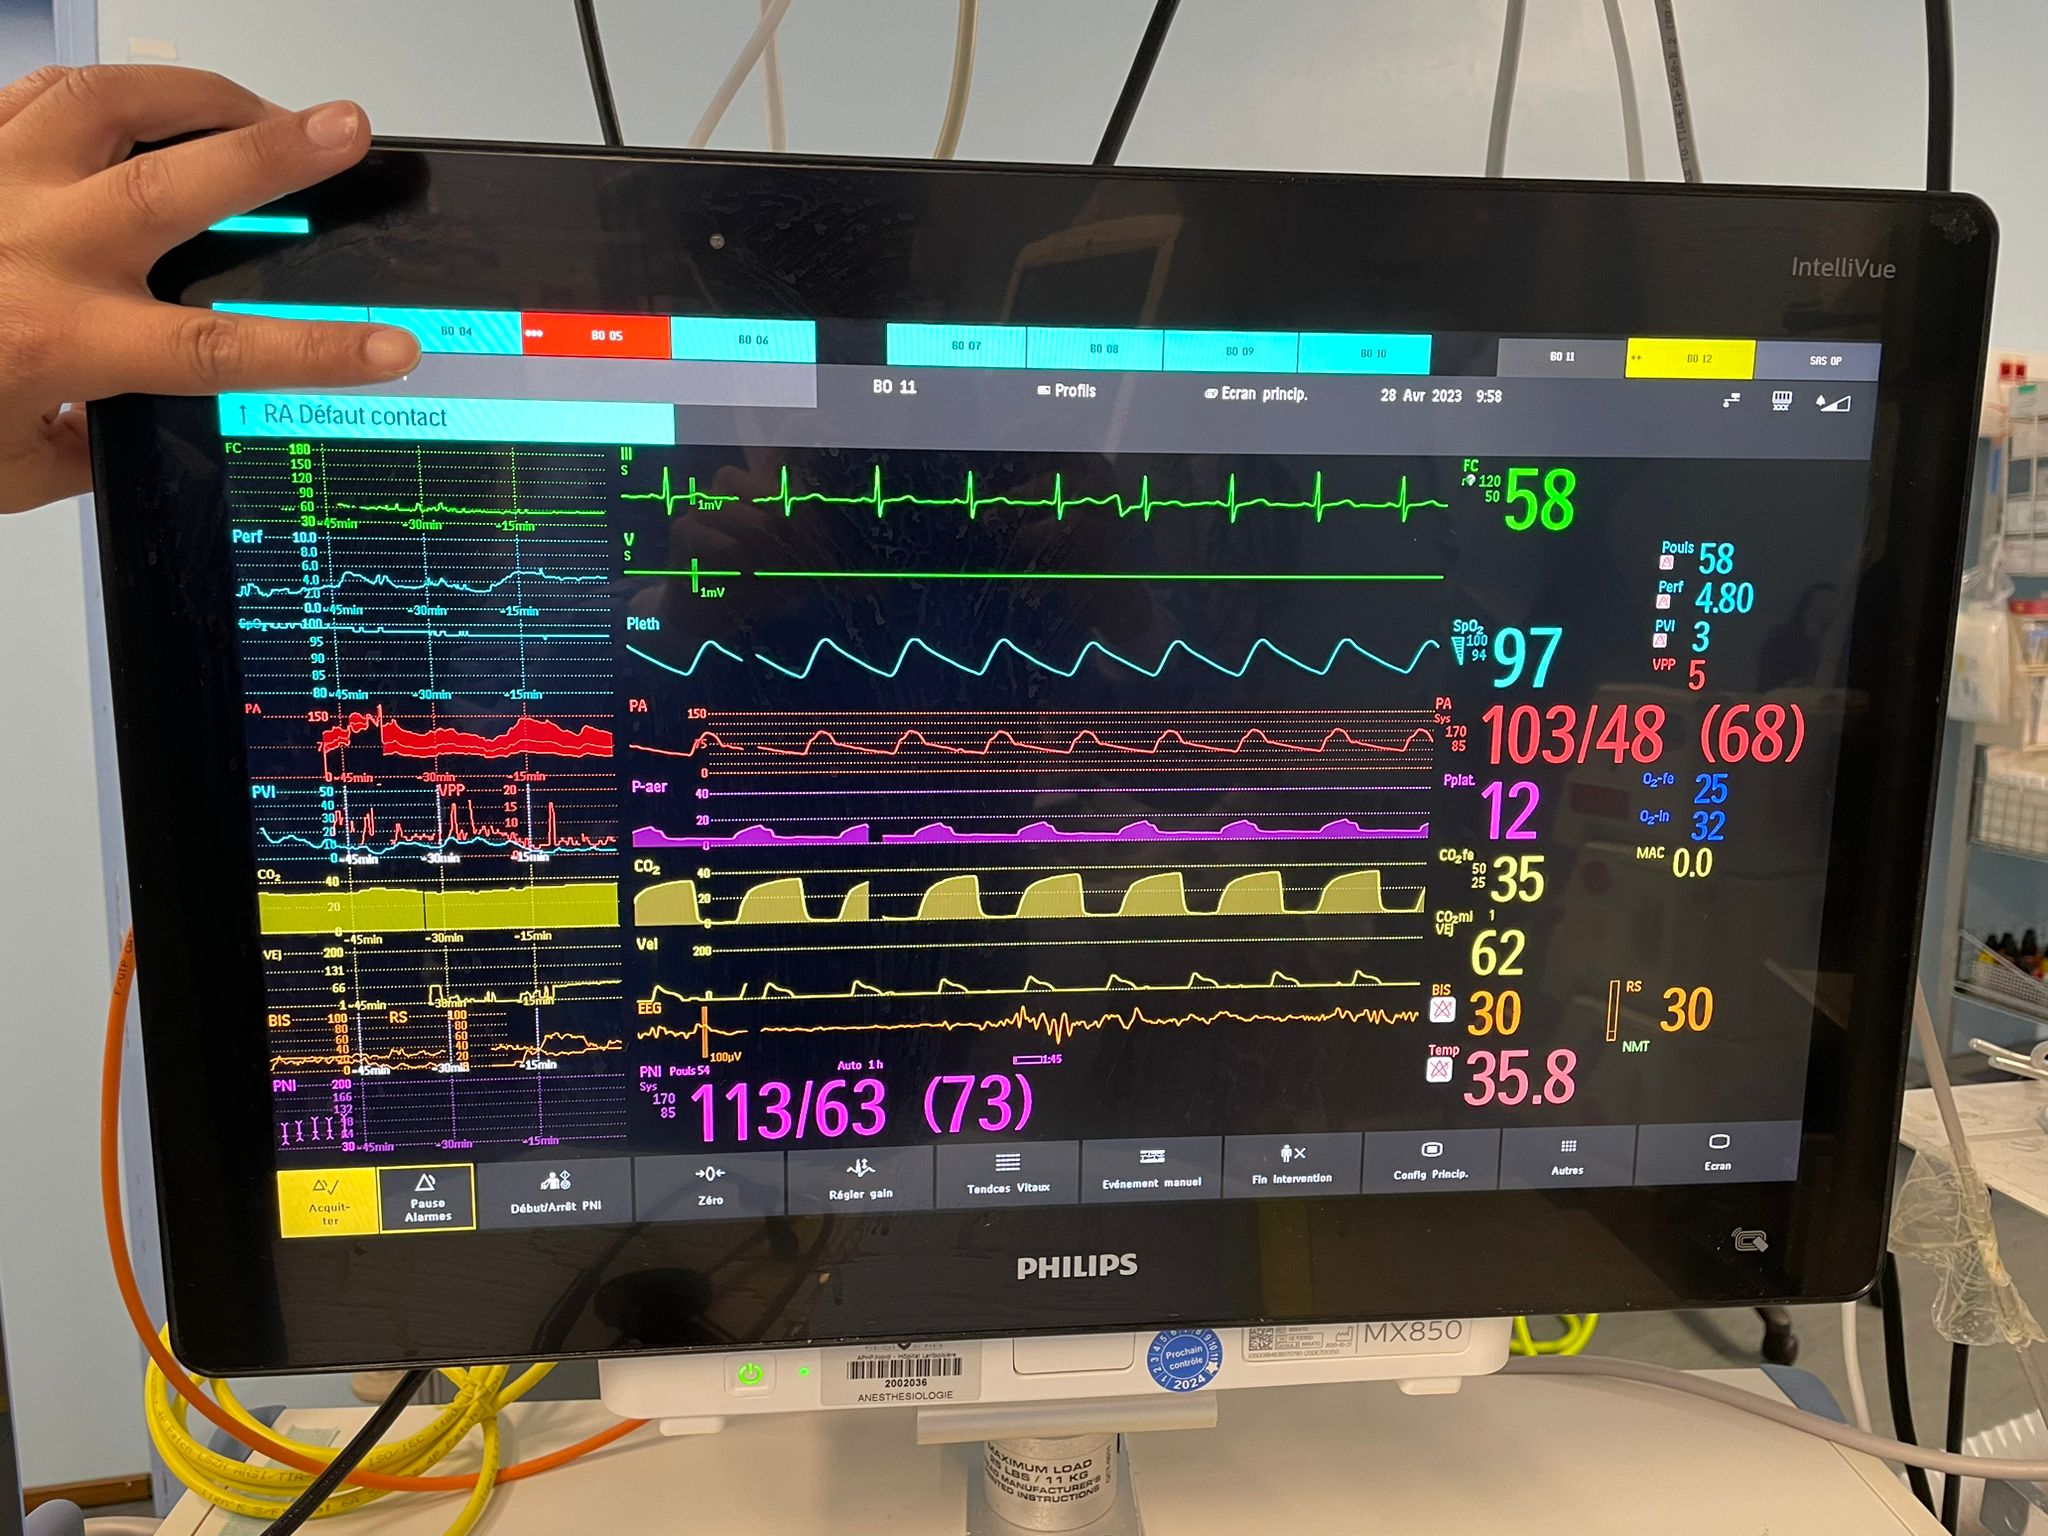
\includegraphics[
            width=1.16\paperwidth
        ]{GA_monitor_1}
    \end{picture}
}
\frame{
    \frametitle{General Anesthesia recordings}


    \begin{tikzpicture}[overlay, remember picture]
            \node[anchor=center, white, xshift=-32ex, yshift=-6em] at (current page.north) (ECG) {\highlight[shadow=false]{\Large \bf ECG}};
            \node[anchor=center, white, xshift=-13ex, yshift=-7.5em] at (current page.north) (ECG_head) {};
            \draw[->, very thick, white] (ECG.east) -- (ECG_head);

            \node[anchor=center, white, xshift=-32ex, yshift=-9.5em] at (current page.north) (Pleth) {\highlight[shadow=false]{\Large \bf Pleth.}};
            \node[anchor=center, white, xshift=-11ex, yshift=-10.5em] at (current page.north) (Pleth_head) {};
            \draw[->, very thick, white] (Pleth.east) -- (Pleth_head);

            \node[anchor=center, white, xshift=-32ex, yshift=-13.5em] at (current page.north) (Resp) {\highlight[shadow=false]{\Large \bf Resp.}};
            \node[anchor=center, white, xshift=-7ex, yshift=-15em] at (current page.north) (Resp_head) {};
            \draw[->, very thick, white] (Resp.east) -- (Resp_head);

            \node[anchor=center, white, xshift=-32ex, yshift=-16.5em] at (current page.north) (EEG) {\highlight[shadow=false]{\Large \bf EEG}};
            \node[anchor=center, white, xshift=-5ex, yshift=-17.5em] at (current page.north) (EEG_head) {};
            \draw[->, very thick, white] (EEG.east) -- (EEG_head);
            \node[anchor=north west, xshift=18ex, yshift=-6em] at (current page.north) {
                \highlight[shadow=false]{Indicators}
            };

    \end{tikzpicture}
}
}

\frame{
    \frametitle{AI-powered General Anesthesia}

    \begin{columns}
        \column{.4\textwidth}
        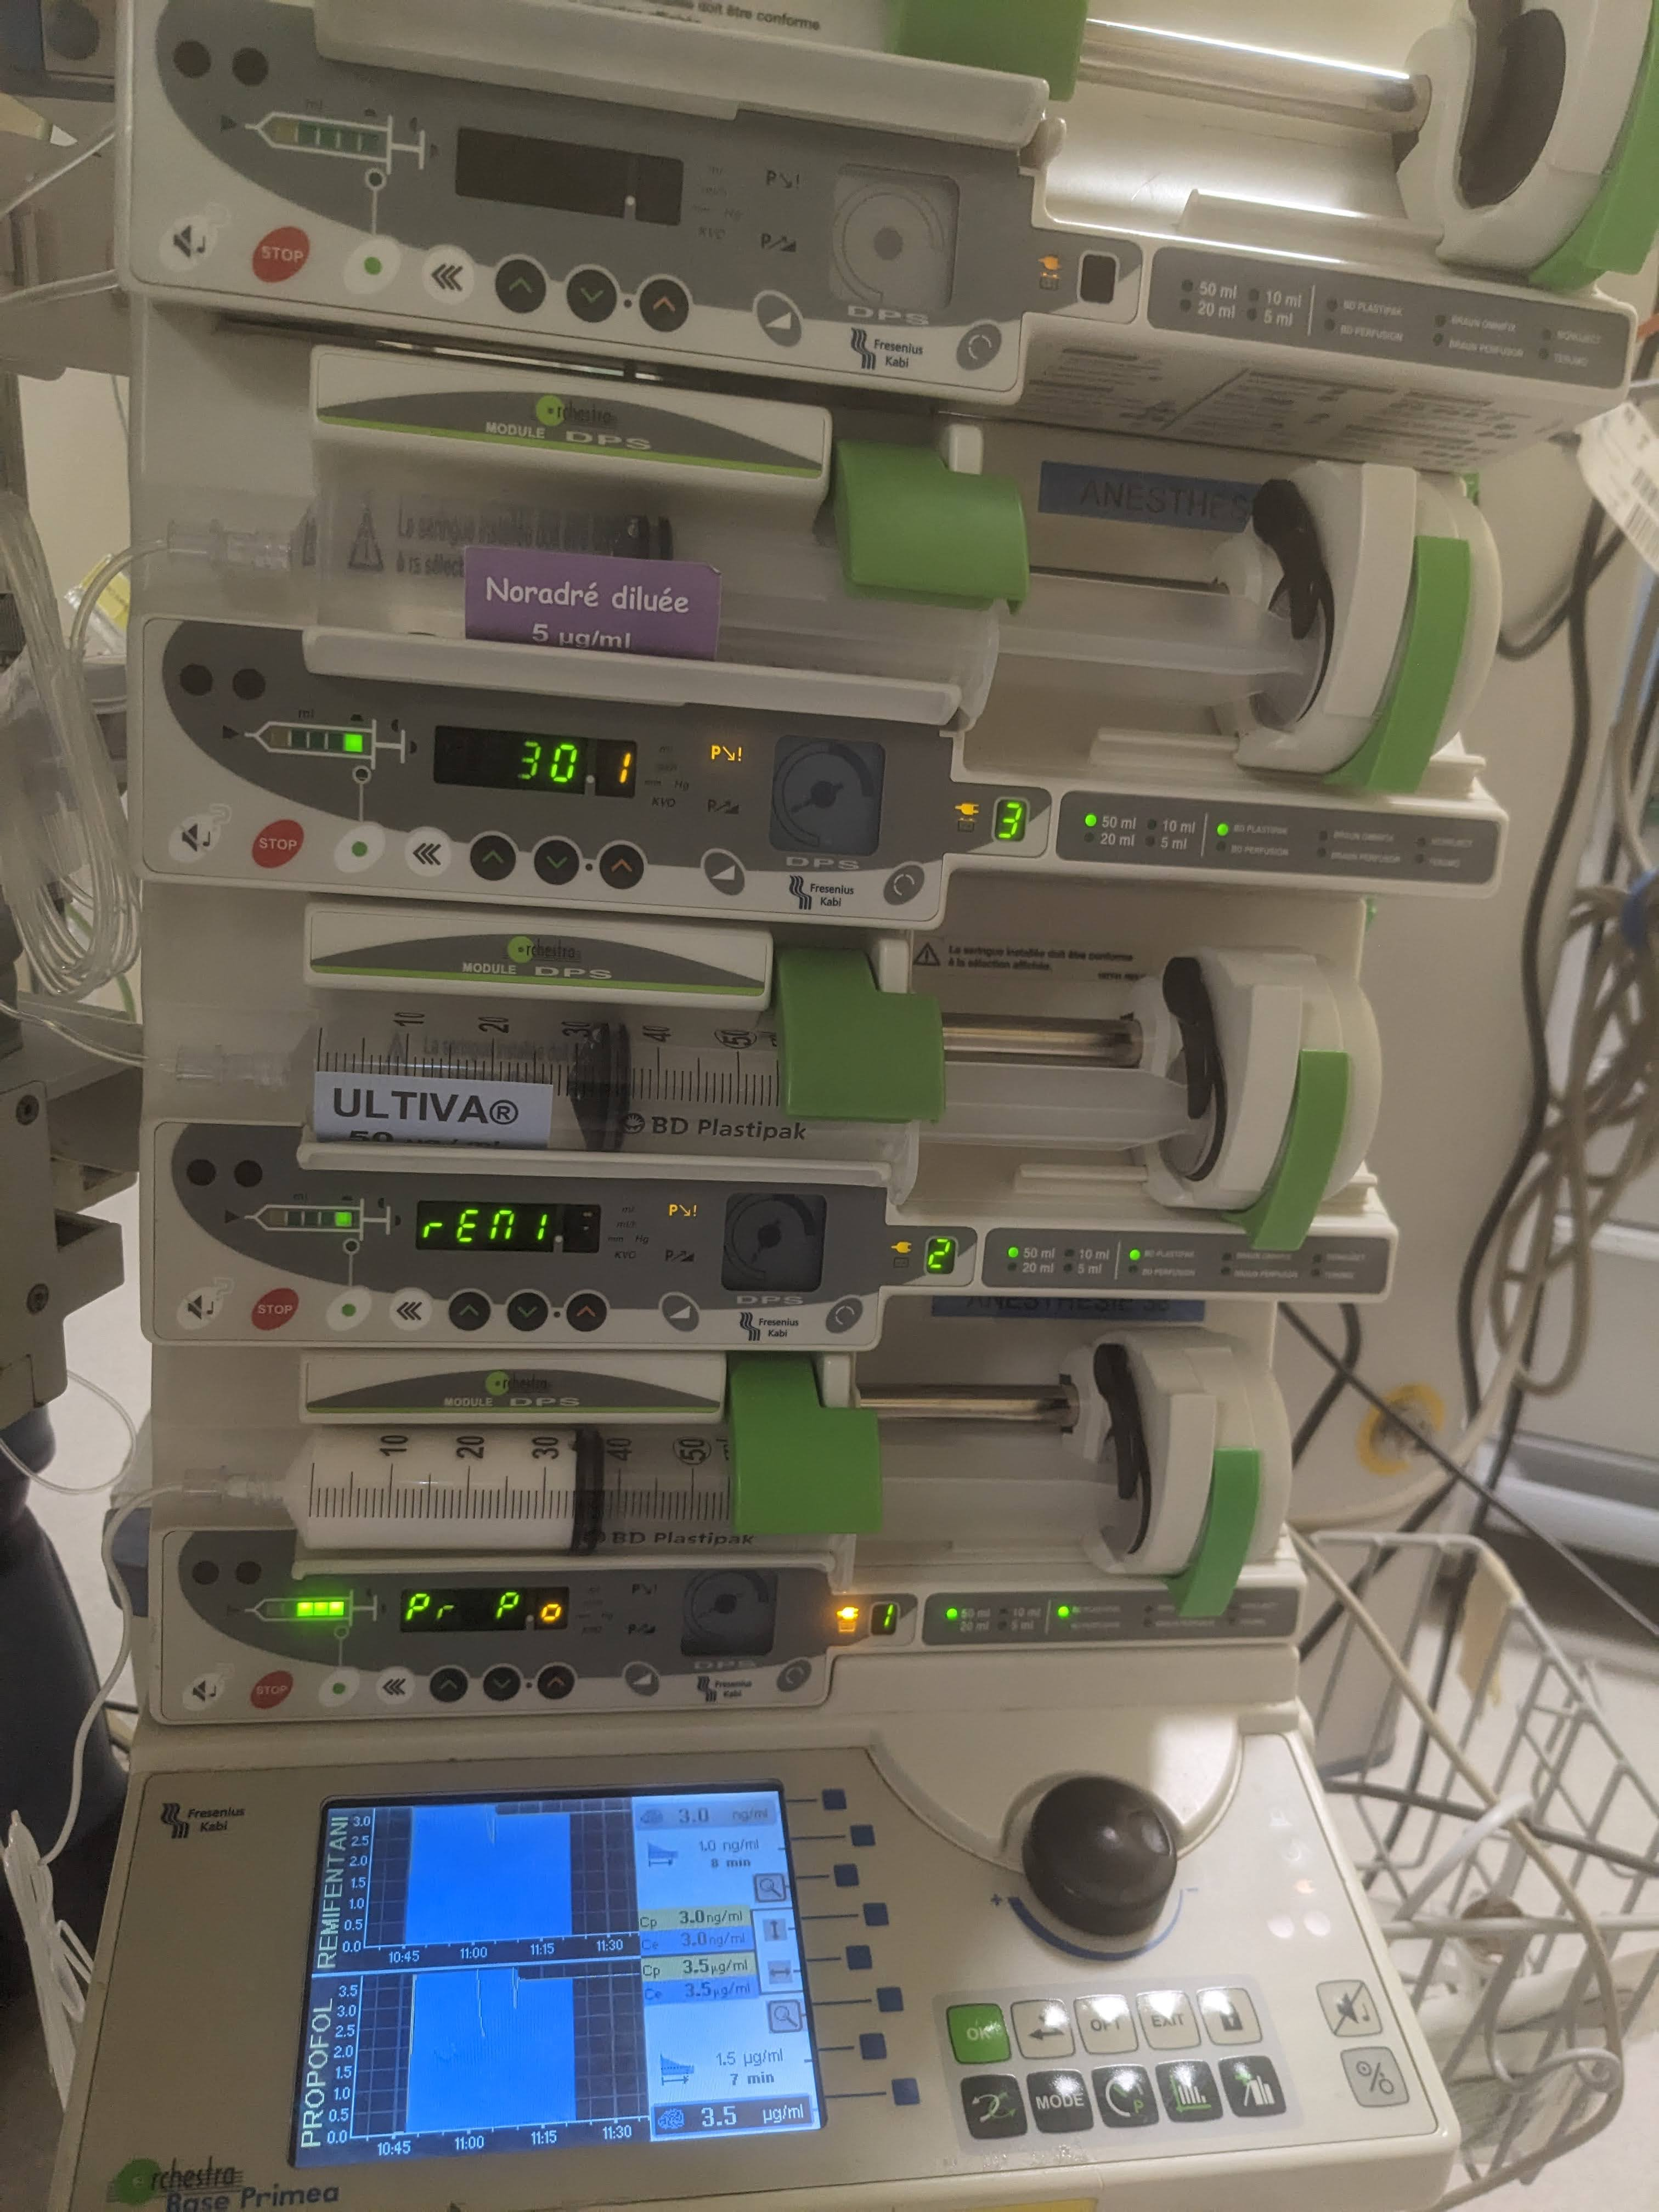
\includegraphics[width=\textwidth]{seringe1}
        \column{.6\textwidth}
        Anesthetists make {\bf decisions} based on these indicators.\\[1em]

        \begin{itemize}\itemsep.5em
            \color{black}\normalfont
            \item Instantaneous snapshot,
            \item Reading needs expertise,
            \item Not personalized.
        \end{itemize}
        \vskip1em
        F. Vallée and the MASCOT team from LAriboisière (hospital in Paris) have been collecting GA recordings for 5 years.
        \vskip2em
        \strongpoint{Can we leverage AI to better drive GA?}
    \end{columns}


}

%------------------------------------------------------------------------------
\frame[t]{
    \frametitle[t]{Recent successes in AI: Foundation Models}

    \begin{columns}[T]
        \column{.2\textwidth}\centering
        
\includegraphics[height=4em]{logo_chatGPT}\\
        \textbf{ChatGPT}
        \column{.2\textwidth}\centering
        
\includegraphics[height=4em]{logo_copilot}\\
        \textbf{Copilot}
        \column{.2\textwidth}\centering
        
\includegraphics[height=4em]{logo_midjourney}\\
        \textbf{Midjourney}
    \end{columns}
    \vskip1em
    {\centering \large What do they have in common?\\}

    \pause

    \vskip1em
    \begin{columns}[T]
        \techterm{Unsupervised Pretraining}
        \techterm{Transformers}
        \techterm{Fine-tuning}
    \end{columns}
    \vskip1em
    \myitem{} Characterize $\mathbb P(X)$ through interaction between {\bf tokens}.

    \only<3>{
        \vskip1em
        {\bf Challenges for signals:}\\[1em]
        \begin{itemize}\itemsep.5em
            \item Databases are smaller than Text and Images,
            \item What are the tokens for the physiological signals?
        \end{itemize}
    }


}

%------------------------------------------------------------------------------
{
\usebackgroundtemplate{
    \begin{picture}(400, 300)(45, 0)
        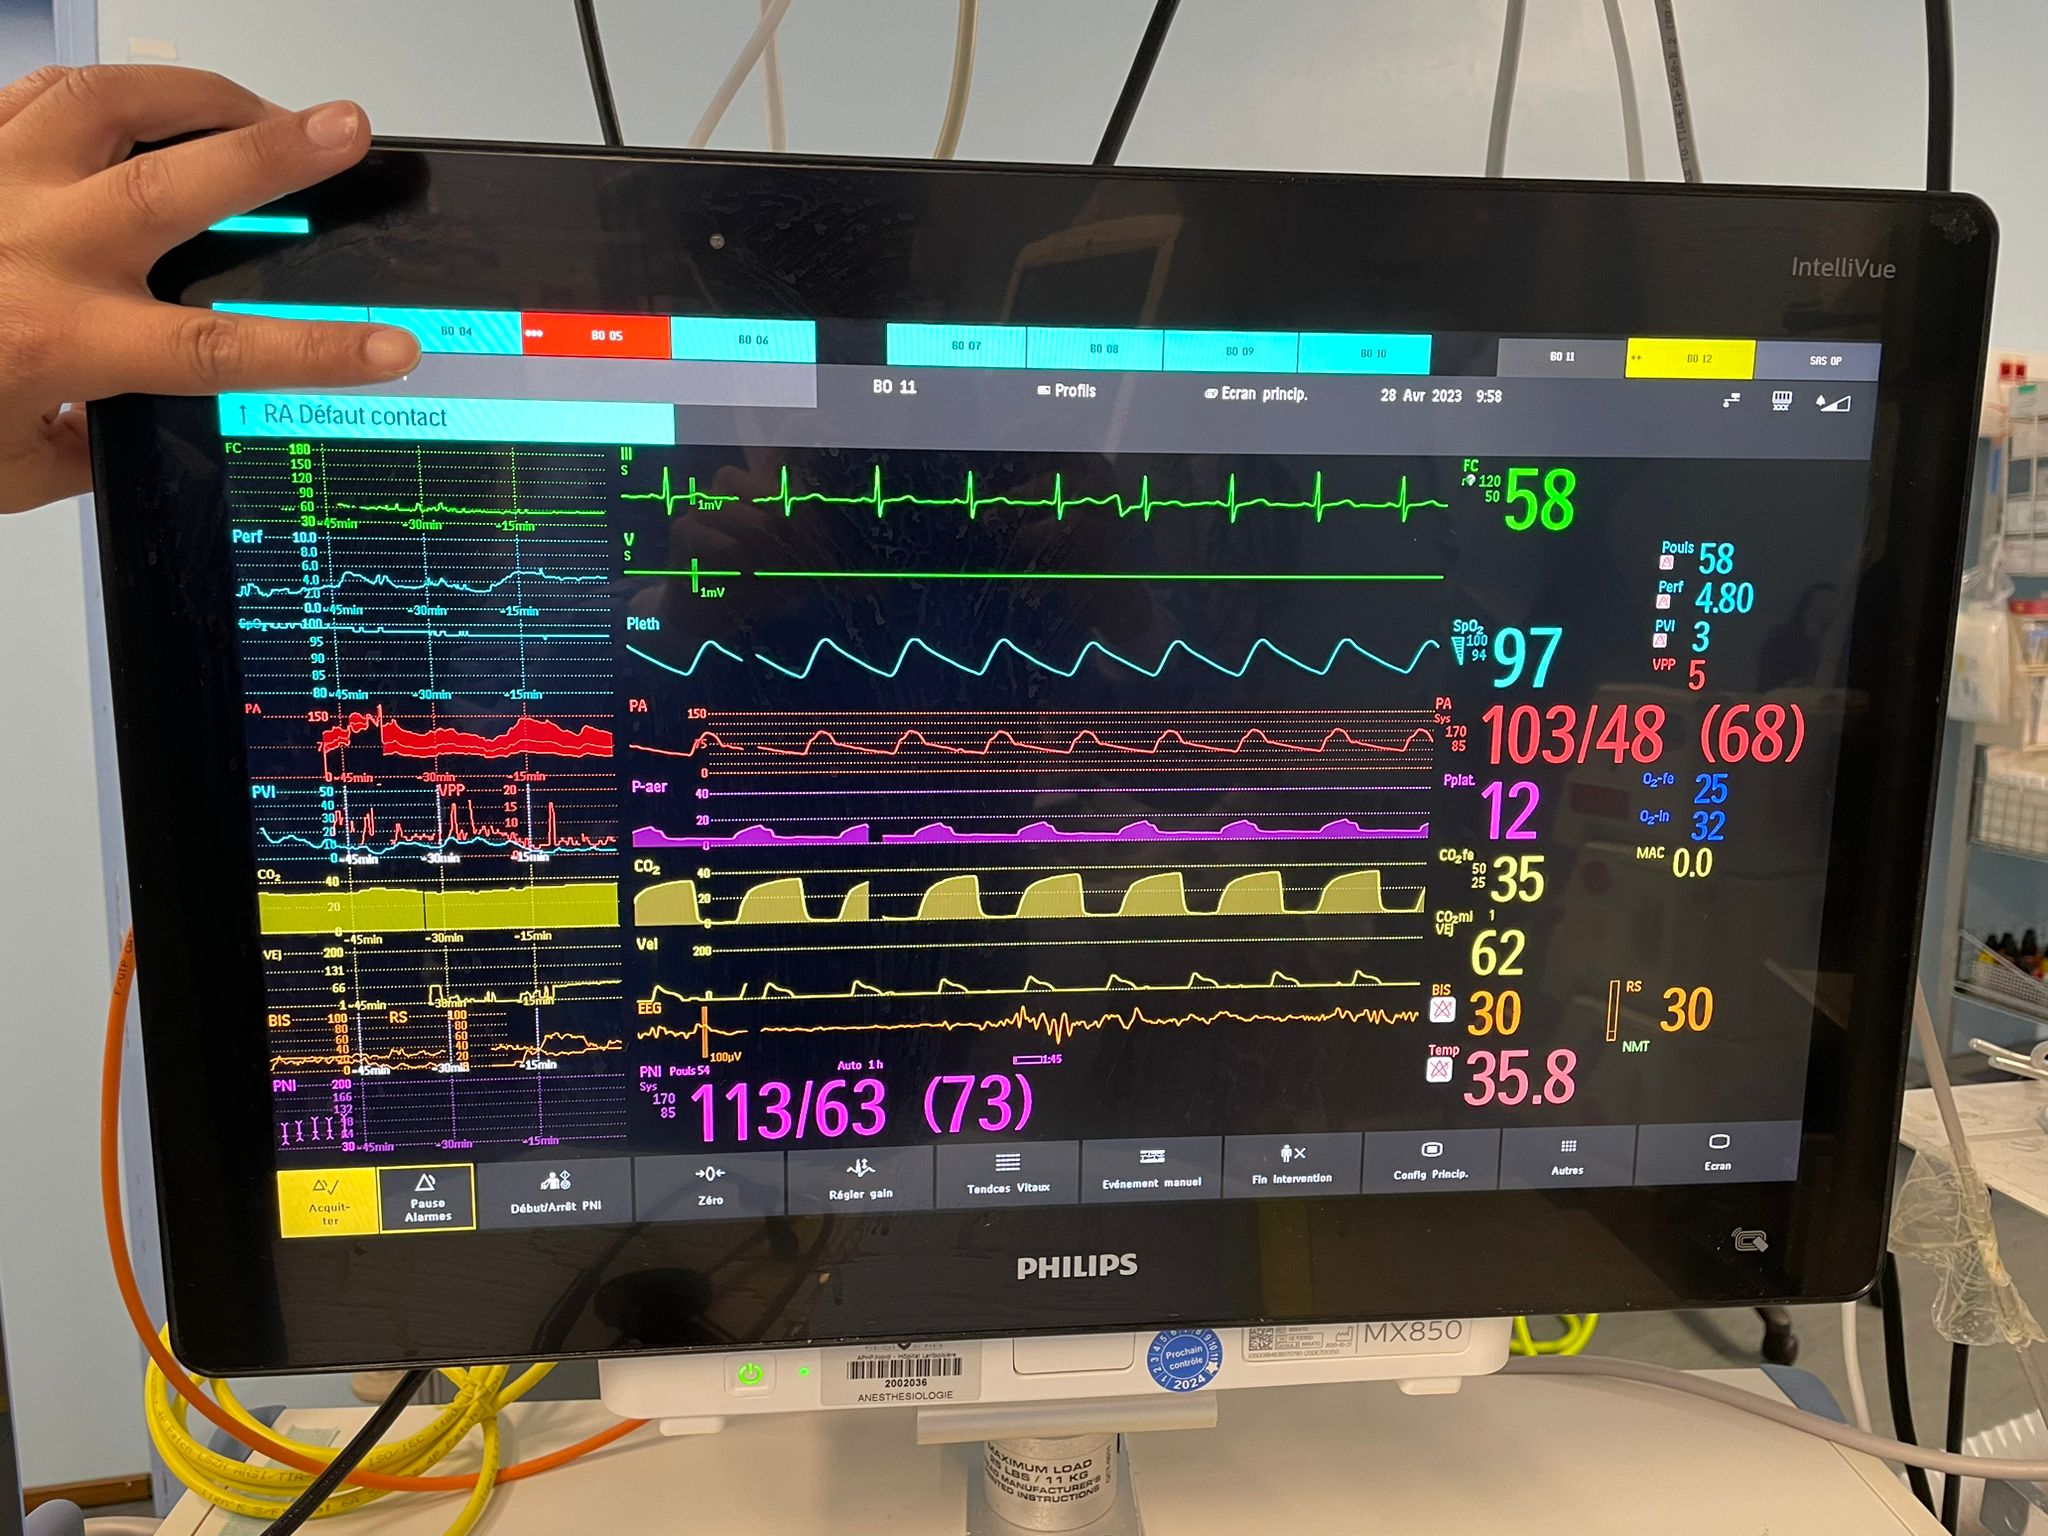
\includegraphics[
            width=1.16\paperwidth
        ]{GA_monitor_1}
    \end{picture}
}
\frame{
    \frametitle{Signals' tokens: Patterns and Events}


    \begin{tikzpicture}[overlay, remember picture]

        \node[anchor=west, yshift=7em] at (current page.west)
            (patterns) {\highlight[shadow=false]{Signal's patterns}};

        \node[anchor=west, yshift=-2.5em] at (patterns.west) (ECG) {\highlight[shadow=false]{\color{black}\normalfont Heartbeat}};
        \node[anchor=center, white, xshift=-13ex, yshift=-7.5em] at (current page.north) (ECG_head) {};
        \draw[->, very thick, white] (ECG.east) -- (ECG_head);

        \node[rectangle, white, draw=white, very thick,
            minimum width=5ex,
            minimum height=2em, xshift=-9ex, yshift=-7.8em]
                at (current page.north) {};

        \node[anchor=west, yshift=-5em] at (patterns.west) (Pleth) {\highlight[shadow=false]{\color{black}\normalfont  Dicrote}};
        \node[anchor=center, white, xshift=-9ex, yshift=-10.5em] at (current page.north) (Pleth_head) {};
        \draw[->, very thick, white] (Pleth.east) -- (Pleth_head);

        \node[rectangle, white, draw=white, very thick,
            minimum width=4ex,
            minimum height=2em, xshift=-7ex, yshift=-10.8em]
                at (current page.north) {};

        \node[anchor=west, yshift=-7.5em] at (patterns.west) (Resp) {\highlight[shadow=false]{\color{black}\normalfont  Cycle}};
        \node[anchor=center, white, xshift=-8ex, yshift=-15em] at (current page.north) (Resp_head) {};
        \draw[->, very thick, white] (Resp.east) -- (Resp_head);

        \node[rectangle, white, draw=white, very thick,
            minimum width=4ex,
            minimum height=2em, xshift=-6ex, yshift=-15.5em]
                at (current page.north) {};

        \node[anchor=west, yshift=-10em] at (patterns.west) (EEG) {\highlight[shadow=false]{\color{black}\normalfont  Brain waves}};
        \node[anchor=center, white, xshift=-5ex, yshift=-17.5em] at (current page.north) (EEG_head) {};
        \draw[->, very thick, white] (EEG.east) -- (EEG_head);

        \node[rectangle, white, draw=white, very thick,
            minimum width=6ex,
            minimum height=1.3em, xshift=-2ex, yshift=-17.8em]
                at (current page.north) {};




        \node[anchor=east, xshift=-3em, yshift=7em] at (current page.east)
            (events) {\highlight[shadow=false]{External events}};
        \node[anchor=east, yshift=-2.5em] at (events.east)
            {\highlight[shadow=false]{\color{black}\normalfont Drug injection}};
        \node[anchor=east, yshift=-5em] at (events.east)
            {\highlight[shadow=false]{\color{black}\normalfont Surgery acts}};
        \node[anchor=east, yshift=-7.5em] at (events.east)
            {\highlight[shadow=false]{\color{black}\normalfont Wakeup}};
        \node[anchor=east, yshift=-10em] at (events.east)
            {\highlight[shadow=false]{\color{black}\normalfont Death}};

        \only<2>{

        \node[anchor=west, yshift=-8em] at (current page.west)
        {\highlight[shadow=false]{Physiological events}};
        }

    \end{tikzpicture}
}
}


%------------------------------------------------------------------------------

\begin{frame}[t]{Signals' tokens: Events}

    \vskip-1em
    \begin{columns}[T]
        \column{.5\textwidth}
        \centering
        \overimg[.9\linewidth]{1}{meg_signal}{2}{meg_dict}\\
        {\large MEG}\\
        \overimg[\linewidth]{1}{Hubble}{2}{Hubble_dict}\\
        {\large Astronomy}\\
    \column{.5\textwidth}
        \centering
        \overimg[\linewidth]{1}{accelero}{2}{accelero_dict}\\
        {\large Gait analysis}\\
        \overimg[.9\linewidth]{1}{tokamak}{2}{tokamak_dict}\\
        {\large Plasma Simulation}\\

    \end{columns}

    \visible<2>{\vskip-12em
    \centering
    \highlight{\parbox{.4\textwidth}{
        \centering
        Physical Signals\\
        composed of
        Reccuring Patterns \& Events
    }}\\
    }
\end{frame}


%------------------------------------------------------------------------------

\frame{
    \frametitle{EULPS: Event-based unsupervised learning for Physiological Signals}

    {\bf Hyp.:} Events' time distribution $\mathbb P(\{t_k\}_k)$ is much simpler than $\mathbb P(X)$.\\[1em]

    % {\bf Two roads:}
    % \begin{columns}[T]
    %     \column{.5\textwidth}
    %     {\centering\highlight{Deep Learning}\\}
    %     \vskip.5em
    %     \begin{itemize}
    %         \item Very expressive,
    %         \item Require very large database,
    %         \item Black-box.
    %     \end{itemize}
    %     \column{.5\textwidth}
    %     {\centering\highlight{Parametric Model}\\}
    %     \vskip.5em
    %     \begin{itemize}
    %         \item Limited fine-tuning,
    %         \item Sample efficient,
    %         \item Explicit.
    %     \end{itemize}
    % \end{columns}

    % \strongpoint{From parametric to deep models}

    % TODO: here I need to explain the issue!!

    \begin{block}{\bf EBUL Goal}
        Model Physiological Signals as the distribution of its Events.
    \end{block}

    \vskip1em
    {\bf Challenge:} Need to find events and model their distribution jointly.\\[1em]

    {\centering
\includegraphics[width=.8\textwidth]{finding_events}\\[1em]}

    {\bf Approach:} from parametric to deep models.
}

%------------------------------------------------------------------------------

\frame{
    \frametitle{WP1: Parametric PP to model Physiological Signals Events}

    \begin{block}{\bf Challenge 1}
        Which parametric models for Physiological Signals Events?
    \end{block}

    {\bf Idea:} model the events' distribution $\mathbb P(\{t_k\}_k)$ with Point Processes (PP)\\[1em]

    \begin{columns}
        \column{.6\textwidth}
        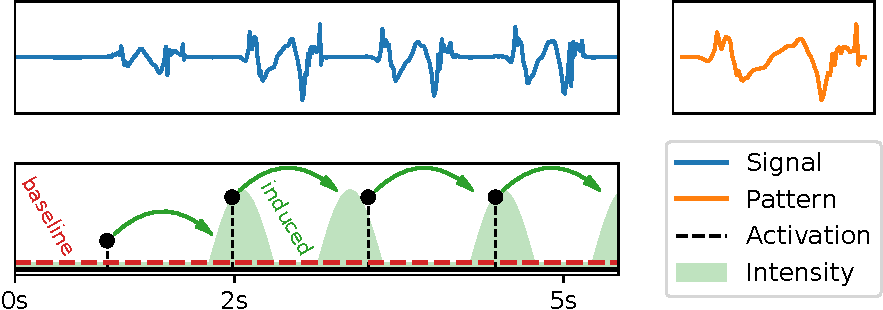
\includegraphics[width=\textwidth]{csc_and_pp}\\
        \column{.4\textwidth}
        \includegraphics[width=\textwidth]{connectivity_default_mode}
    \end{columns}

    \vskip1em
    {\bf Expected Results:}\\
    \myitem{} General Parametric Family for temporal, marked and spatial PP.

    \vskip1em
    {\bf Preliminary Studies:} \fakecite{ICLR 2022; ICML 2023}

}

%------------------------------------------------------------------------------

\frame{
    \frametitle{WP2: Event-based unsupervised waveform learning\\for physiological signals}

    \begin{block}{\bf Challenge 2}
        Can we jointly discover the Events and model them?
    \end{block}

    \begin{columns}[T]
        \column{.5\textwidth}
        {\centering
        \highlight{Parametric models}\\[1em]}
        \begin{itemize}
            \item Based on Convolutional Dictionary Learning and PP,
            \item Use bilevel optimization.
        \end{itemize}
        \column{.5\textwidth}
        {\centering
        \highlight{Deep Learning models}\\[1em]}
        \begin{itemize}
            \item Architecture based on parametric models unrolling,
            \item Fully differentiable.
        \end{itemize}
    \end{columns}

    \vskip2em
    {\bf Expected Results:}\\[.5em]
    \myitem{} Methods to build joint representations for signal and events.\hfill

    \vskip1em
    {\bf Preliminary Studies:} \fakecite{ICLR 2022a; NeurIPS 2022}
}

%------------------------------------------------------------------------------

\frame{
    \frametitle{WP3: Validating representations with practical tasks}

    \begin{block}{\bf Challenge 3}
        Develop methods to impact GA with fine-tuned models using $\mathbb P(\{t_k\}_k)$.
    \end{block}

    {\bf Idea:} Leverage likelihood and differentiable architecture.

    \vskip1em
    {\bf Expected Results:} Data processing for GA and Neurosciences.\\[1em]
    \begin{columns}[T]
        \techterm{Event Prediction}
        \techterm{Anomaly Detection}
        \techterm{Causality}
    \end{columns}\vskip1em
    \begin{columns}[T]
        \column{.3\textwidth}
        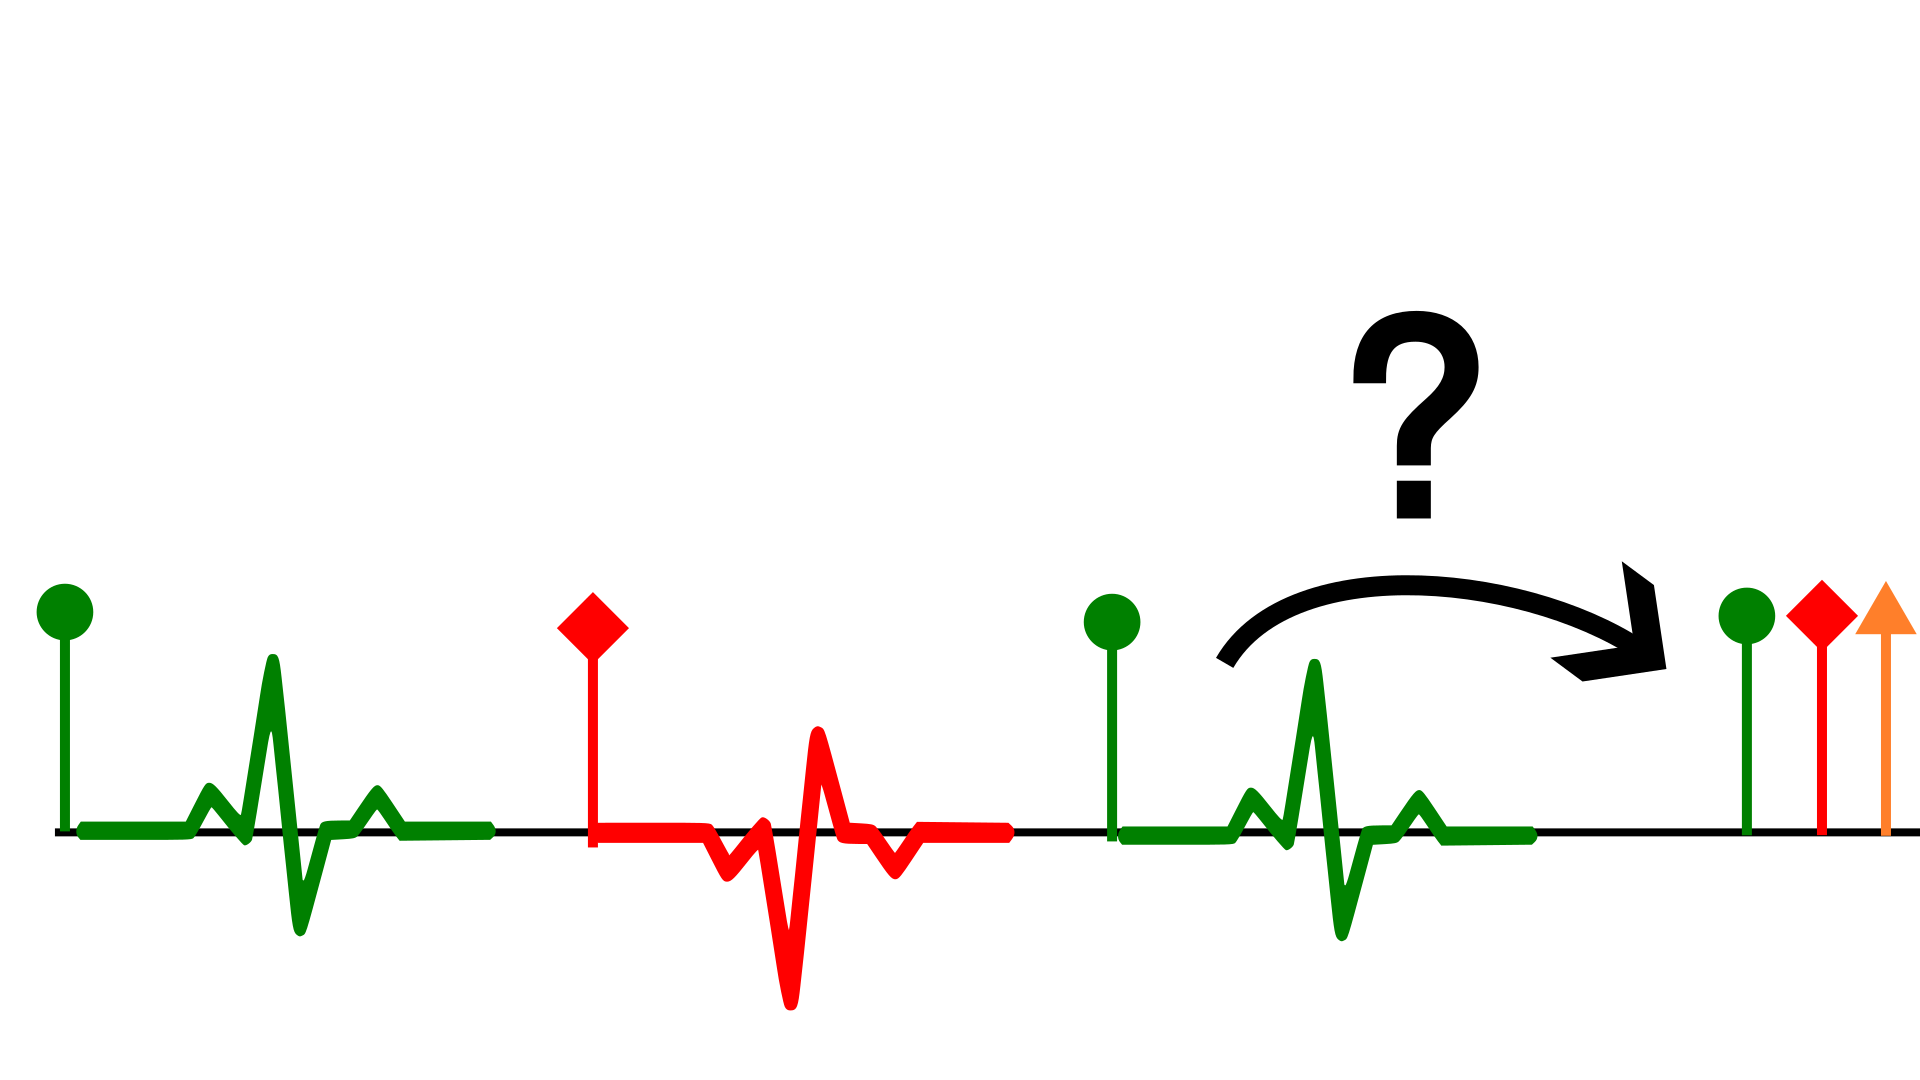
\includegraphics[width=\textwidth]{forecasting}
        \column{.3\textwidth}
        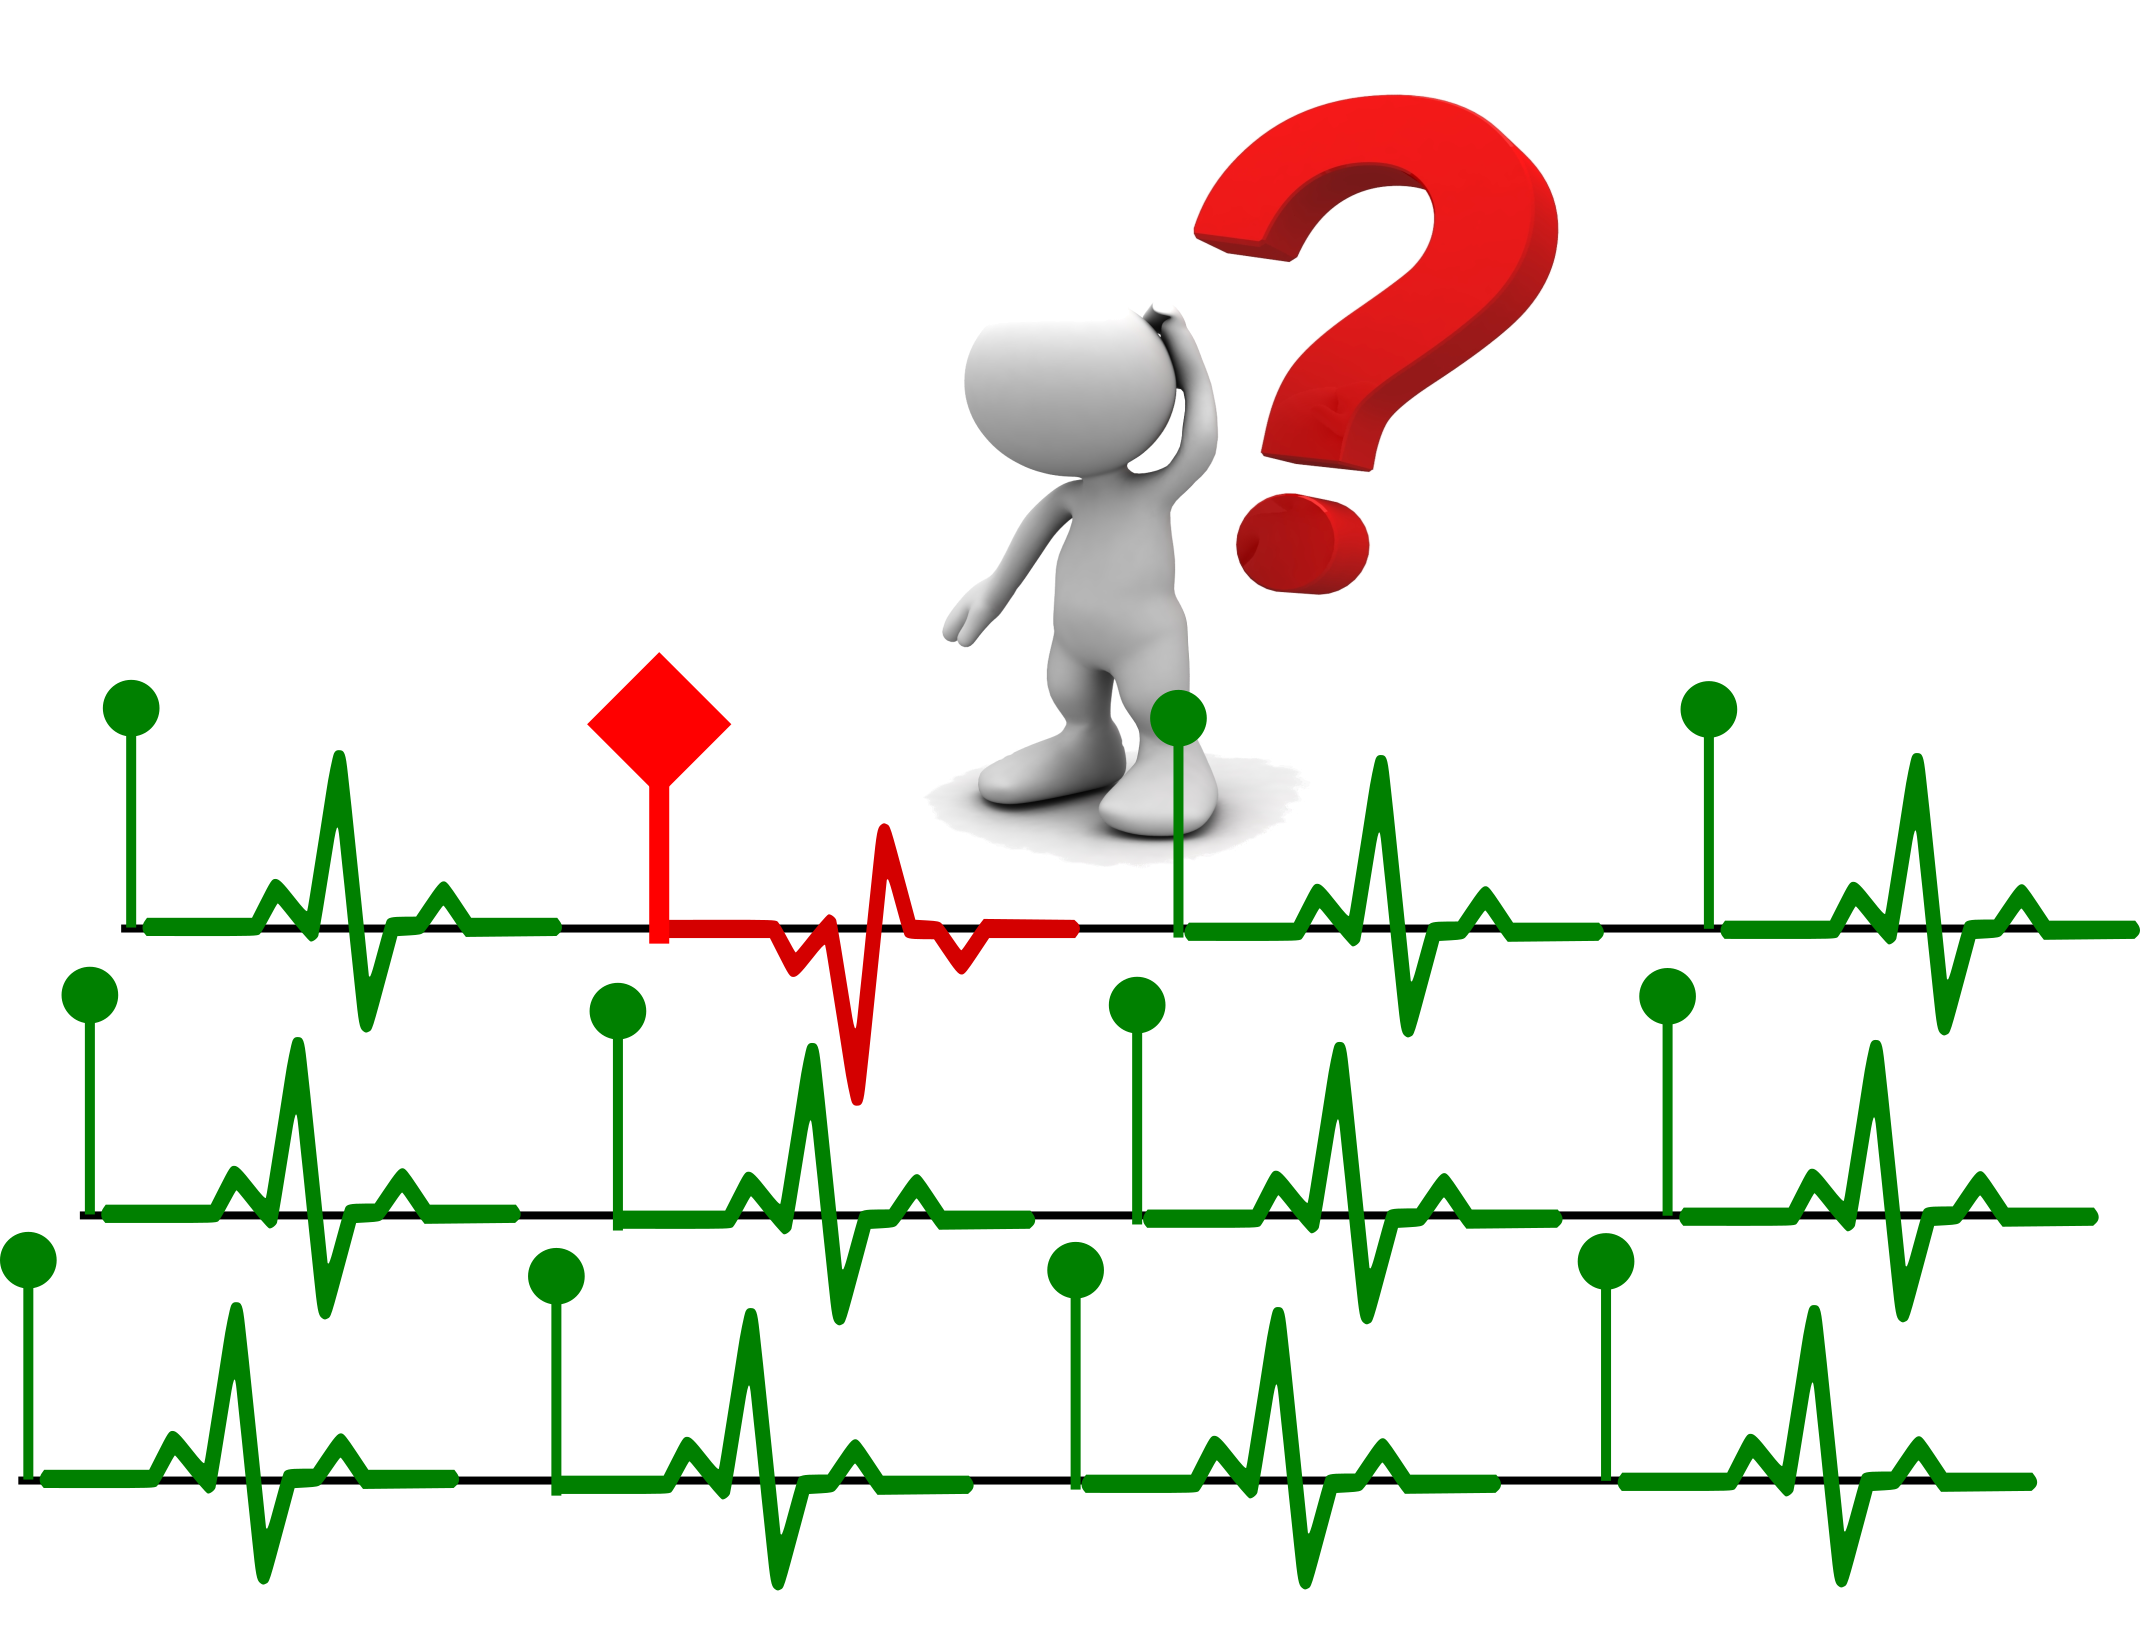
\includegraphics[width=1\textwidth]{anomaly_detection}
        \column{.3\textwidth}
        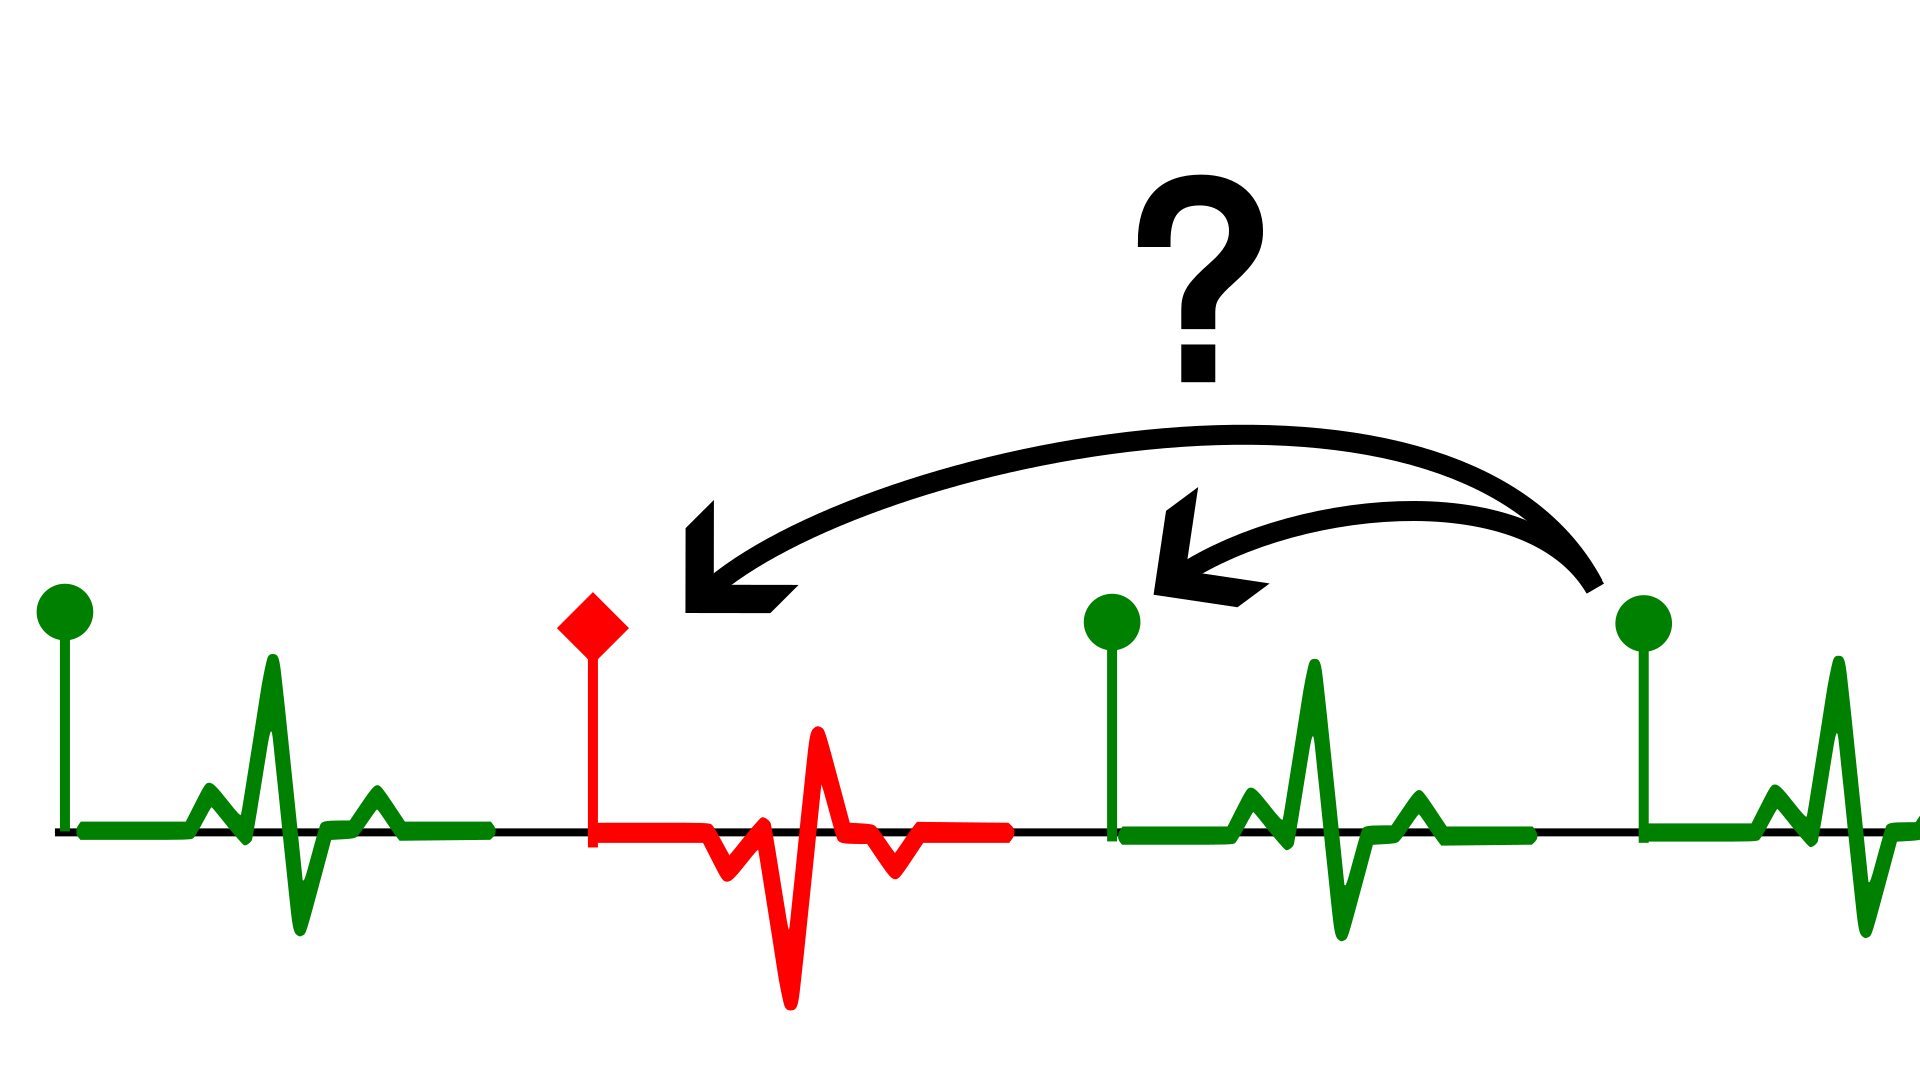
\includegraphics[width=\textwidth]{images/causality.png}
    \end{columns}

}

%------------------------------------------------------------------------------

% \frame{
%     \frametitle{WP4: Reproducible and Reusable Research}

%     \begin{block}{\bf Challenge 4}
%         Disseminate these techniques.
%     \end{block}

% }

%------------------------------------------------------------------------------

\frame[t]{
    \frametitle{Principal Investigator: Thomas Moreau}

    % {\bf Carrier Path:}\\[.5em]
    % \highlightbox{\parbox{.9\textwidth}{
    %     \begin{tabular}{c p{2ex} l p{2ex} c}
    %         {\bf\color{black} 2014-2017}&&PhD && ENS Cachan\\
    %         {\bf\color{black} 2018-2019}&&Postdoc && Inria\\
    %         {\bf\color{black} 2019-Present}&&Research faculty&& Inria\\

    %     \end{tabular}

    % }}
    \begin{block}{\bf Goal}
        Model Physiological Signals as the distribution of its Events.
    \end{block}
    \vskip1em

    {\bf Impact:} New road for signals processing.\\[.5em]

    % tikz figure with 3 circles linked with arrows going forward and backward and the the following text in each circle:
    % - Core ML
    %- Applications
    % - Software
    \begin{tikzpicture}[overlay, remember picture]

        \node[anchor=south, xshift=-12ex, yshift=9em] at (current page.south) (cloud_ML) {
\includegraphics[width=15ex]{cloud}};
        \node[anchor=north, yshift=.7em] at (cloud_ML) (ML) {Core ML\phantom{p}};
        \node[anchor=south, xshift=12ex, yshift=9em] at (current page.south) (cloud_app) {
\includegraphics[width=15ex]{cloud}};
        \node[anchor=north, yshift=.3em] at (cloud_app) (App) {Applications};
        \node[anchor=south, yshift=2em] at (current page.south) (cloud_soft) {
\includegraphics[width=15ex]{cloud}};
        \node[anchor=north, yshift=.7em] at (cloud_soft) (Soft) {Software\phantom{p}};
        \node[anchor=south, yshift=7em] at (current page.south) {\parbox{.15\textwidth}{\centering \bf \color{darkred} Thomas Moreau}};

        \draw[-latex] (cloud_app) to[bend right=5] node[above,rotate=60] {} (cloud_ML);
        \draw[-latex] (cloud_ML) to[bend right=5] node[above,rotate=60] {} (cloud_app);
        \draw[-latex] (cloud_app) to[bend right=5] node[above,rotate=60] {} (cloud_soft);
        \draw[-latex] (cloud_soft) to[bend right=5] node[above,rotate=60] {} (cloud_app);
        \draw[-latex] (cloud_soft) to[bend right=5] node[above,rotate=60] {} (cloud_ML);
        \draw[-latex] (cloud_ML) to[bend right=5] node[above,rotate=60] {} (cloud_soft);

        \node[anchor=east, xshift=-20ex, yshift=-2ex] at (cloud_soft.west) {\includegraphics[height=1.5em]{logo_python}};
        \node[anchor=east, xshift=-12ex, yshift=-2ex] at (cloud_soft.west) (sklearn){\includegraphics[height=1.5em]{logo_sklearn}};
        \node[anchor=south, xshift=-3ex, yshift=-1ex] at (sklearn.north) {\footnotesize Contributor};
        \node[anchor=east, xshift=-1ex, yshift=4ex] at (cloud_soft.west) {\includegraphics[height=3em]{logo_joblib}};
        \node[anchor=east, xshift=-1ex, yshift=-3ex] at (cloud_soft.west) {\includegraphics[height=3em]{logo_loky}};
        \node[anchor=west, xshift=-1ex, yshift=4ex] at (cloud_soft.east) {\includegraphics[height=3em]{logo_benchopt}};
        \node[anchor=west, xshift=0ex, yshift=-2ex] at (cloud_soft.east) (alpha) {\includegraphics[height=3em]{brain_and_signals}};
        \node[anchor=north, yshift=1ex] at (alpha.south) {\footnotesize\texttt{{\color{orange}$\pmb\alpha$}csc}};
    \end{tikzpicture}

    \highlight{\parbox[c]{.18\textwidth}{
        2018-2023\\
        \normalfont\color{black} 17 papers in top ML conf.
    }}
    \hfill
    \highlight{\parbox[c]{.2\textwidth}{
        2015-2023\\
        \normalfont\color{black}
        7 journal pub.\\
        1 Patent
    }}\\

}




\appendix

%------------------------------------------------------------------------------
\frame{
    \frametitle{References}

    \footnotesize
    \begin{itemize}\itemindent4em
        \item[\fakecite{ICLR2022}] Allain, C., Gramfort, A. \& {\bf Moreau, T.} \emph{DriPP: Driven Point Process to Model Stimuli Induced Patterns in M/EEF Signals.} in ICLR 2022.
        \item[\fakecite{ICLR2022a}] Malézieux, B., {\bf Moreau, T.} \& Kowalski, M. \emph{Understanding approximate and Unrolled Dictionary Learning for Pattern Recovery.} in ICLR 2022.
        \item[\fakecite{NeurIPS2022}] Dagréou, M., Ablin, P., Vaiter, S. \& {\bf Moreau, T.} \emph{A framework for bilevel optimization that enables stochastic and global variance reduction algorithms.} in NeurIPS 2022.
        \item[\fakecite{ICML2023}] Staerman, G., Allain, C., Gramfort, A. \& {\bf Moreau, T.} \emph{FaDIn: Fast Discretized Inference for Hawkes Processes with General Parametric Kernels.} in ICML 2023.
        \item[\fakecite{NImg 2023}] Power, L., Allain, C., {\bf Moreau, T.}, Gramfort, A. \& Bardouille, T. \emph{Using convolutional dictionary learning to detect task-related neuromagnetic transients and ageing trends in a large open-access dataset.} NeuroImage 2023.

    \end{itemize}
}


%------------------------------------------------------------------------------

\frame{
    \frametitle{EULPS}


    \begin{block}{\bf Goal}
        Model Physiological Signals as the distribution of its Events.
    \end{block}

    \vskip1em
    {\bf Road:} From Parametric to Deep Models.
    \vskip1em
    {\bf Impact:} Physiological \& Physical Signals Processing
    \vskip1em
    {\bf Applications:} General Anesthesia \& Neuroscience
    \vskip1em
    {\bf Team:}\\
    \myitem{} PI, 4 PhDs, 2 post doc, 1 engineer\\
    \myitem{} Local support: point process/bilevel optimization/anesthesia

}


% %------------------------------------------------------------------------------

% \frame{
%     \bibliography{library}
% }

\end{document}